\documentclass[11pt]{report}

\usepackage[a4paper,margin=1in]{geometry}
\usepackage{fancyhdr}
\usepackage{titlesec}
\usepackage{tabularx}
\usepackage{longtable}
\usepackage{booktabs}
\usepackage{graphicx}
\usepackage{tikz}
\usetikzlibrary{shapes.geometric, arrows.meta, positioning, calc}
\usepackage{enumitem}
\usepackage{hyperref}
\usepackage{xcolor}

\definecolor{titlered}{HTML}{9B1C2E}

\titleformat{\chapter}[hang]{\normalfont\Large\bfseries\color{titlered}}{\thechapter.}{10pt}{}
\titleformat{\section}{\normalfont\large\bfseries}{\thesection}{8pt}{}
\titleformat{\subsection}{\normalfont\normalsize\bfseries\itshape}{\thesubsection}{6pt}{}

\pagestyle{fancy}
\fancyhf{}
\fancyhead[L]{Software Requirements Specification}
\fancyhead[R]{Smart Hostel Room Allocation System}
\fancyfoot[C]{\thepage}
\renewcommand{\headrulewidth}{0.4pt}

\hypersetup{
    colorlinks=true,
    linkcolor=black,
    urlcolor=blue,
    citecolor=black,
    pdftitle={Smart Hostel Room Allocation System - SRS}
}

\title{
    \vspace{2cm}
    \textbf{\Large SOFTWARE REQUIREMENTS SPECIFICATION}\\[0.5cm]
    for\\[0.5cm]
    {\Large \textbf{Smart Hostel Room Allocation System}}\\[0.3cm]
    Version 1.0
}
\author{
    Prepared by:\\
    1. Avleen Kaur (1024030403)\\
    2. Rishab Kumar Jha (1024030416)\\
    3. Daksh Kohli (1024030423)\\[0.5cm]
    Submitted to: Mr. Hardik\\[0.3cm]
    Thapar Institute of Engineering and Technology
}
\date{}

\begin{document}

% ---------------- Title Page ----------------
\begin{titlepage}
\maketitle
\thispagestyle{empty}
\end{titlepage}

% ---------------- Table of Contents ----------------
\tableofcontents
\thispagestyle{empty}
\newpage

% ============================================================
\chapter{Introduction}

\section{Purpose}
Hostel administration at the institute already runs on FretBox, which holds student master data and
handles fees, complaints and gate passes. What FretBox does not provide is student-driven room
allocation: rooms are assigned centrally, friend groups coordinate informally over messaging apps,
and students learn their allotment only at check-in. The Smart Hostel Room Allocation System closes
that gap. It draws student and hostel records from FretBox rather than any hand-maintained sheet, and
lets students form groups and self-select clusters inside an automated, rule-governed allocation engine.

\section{Intended Audience and Reading Suggestions}
This SRS is written for faculty evaluators, the student development team, and future maintainers.
Sections 2--3 describe the system functionally; Sections 4--8 give the technical detail needed to
build and maintain it.

\section{Project Scope}
The system allows:
\begin{itemize}[leftmargin=1.2cm]
    \item Students register against their FretBox record, then create or join a group using a group code.
    \item Group leaders browse live cluster availability and submit a ranked list of preferences.
    \item Rooms are allocated automatically to groups and single applicants by availability and preference order.
    \item Every group member must complete fee payment before the booking is confirmed.
    \item Admins can override allocations and monitor bookings and payments.
\end{itemize}

\begin{figure}[h]
\centering
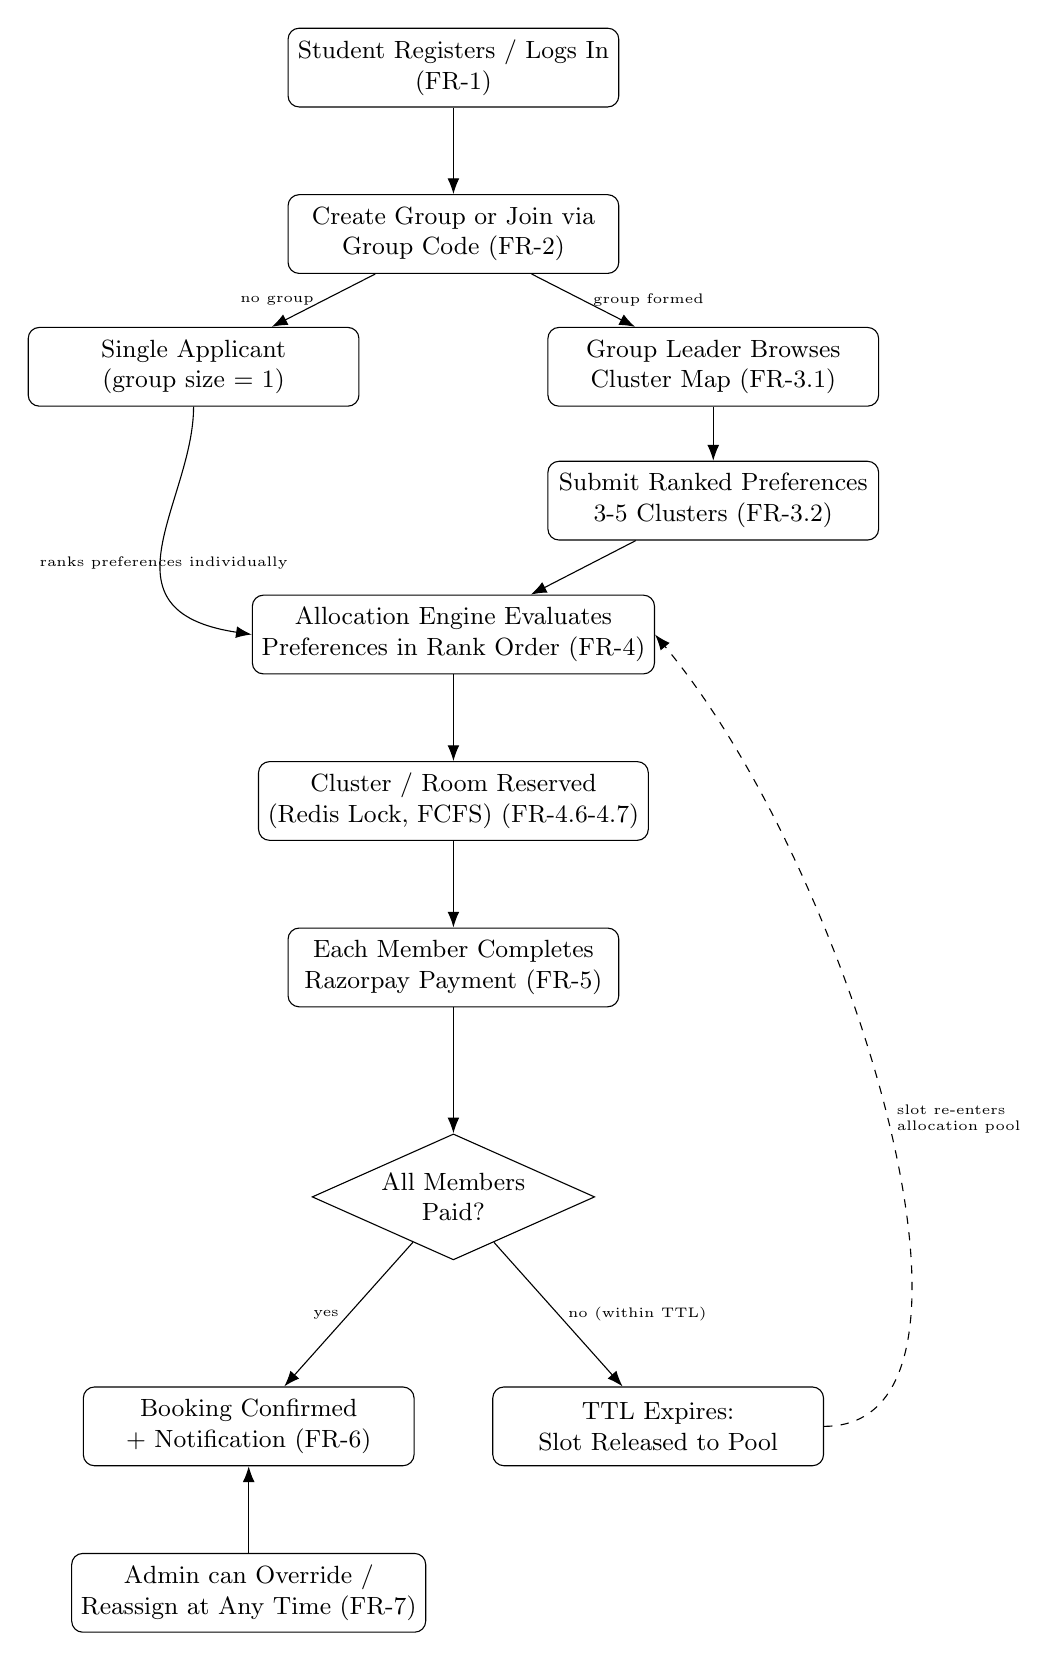
\begin{tikzpicture}[
    box/.style={rectangle, rounded corners, draw=black, minimum width=4.2cm, minimum height=1cm, align=center, font=\small},
    decisionbox/.style={diamond, draw=black, aspect=2.5, align=center, font=\small, inner sep=1pt},
    arrow/.style={-{Latex[length=2mm]}}
]
\node[box] (register) at (0,15) {Student Registers / Logs In\\(FR-1)};
\node[box, below=1.1cm of register] (group) {Create Group or Join via\\Group Code (FR-2)};
\node[box] (single) at (-3.3,11.2) {Single Applicant\\(group size = 1)};
\node[box] (leader) at (3.3,11.2) {Group Leader Browses\\Cluster Map (FR-3.1)};
\node[box] (prefs) at (3.3,9.5) {Submit Ranked Preferences\\3-5 Clusters (FR-3.2)};
\node[box] (engine) at (0,7.8) {Allocation Engine Evaluates\\Preferences in Rank Order (FR-4)};
\node[box, below=1.1cm of engine] (reserved) {Cluster / Room Reserved\\(Redis Lock, FCFS) (FR-4.6-4.7)};
\node[box, below=1.1cm of reserved] (payment) {Each Member Completes\\Razorpay Payment (FR-5)};
\node[decisionbox, below=1.6cm of payment, minimum width=3.2cm, minimum height=1.6cm] (allpaid) {All Members\\Paid?};
\node[box, below=1.6cm of allpaid, xshift=-2.6cm] (confirmed) {Booking Confirmed\\+ Notification (FR-6)};
\node[box, below=1.6cm of allpaid, xshift=2.6cm] (ttl) {TTL Expires:\\Slot Released to Pool};
\node[box, below=1.1cm of confirmed] (admin) {Admin can Override /\\Reassign at Any Time (FR-7)};

\draw[arrow] (register) -- (group);
\draw[arrow] (group) -- node[left, font=\tiny] {no group} (single);
\draw[arrow] (group) -- node[right, font=\tiny] {group formed} (leader);
\draw[arrow] (leader) -- (prefs);
\draw[arrow] (single.south) .. controls +(0,-1.2) and +(-2,0.3) .. node[below, font=\tiny] {ranks preferences individually} (engine.west);
\draw[arrow] (prefs) -- (engine);
\draw[arrow] (engine) -- (reserved);
\draw[arrow] (reserved) -- (payment);
\draw[arrow] (payment) -- (allpaid);
\draw[arrow] (allpaid) -- node[left, font=\tiny] {yes} (confirmed);
\draw[arrow] (allpaid) -- node[right, font=\tiny] {no (within TTL)} (ttl);
\draw[arrow] (admin) -- (confirmed);
\draw[arrow, dashed] (ttl.east) .. controls +(2.5,0) and +(2.5,-3) .. node[right, font=\tiny, align=left] {slot re-enters\\allocation pool} (engine.east);
\end{tikzpicture}
\caption{End-to-end student booking workflow, from registration to confirmed booking.}
\end{figure}

\subsection*{Definitions, Acronyms, and Abbreviations}
\begin{longtable}{p{3.2cm}p{10cm}}
\toprule
\textbf{Term} & \textbf{Definition} \\
\midrule
Cluster & Two rooms sharing a bathroom; total capacity 4 students \\
Room & A 2-seater unit; two rooms per cluster \\
Group & 1--4 students who wish to be housed together, led by a Group Leader \\
FCFS & First-Come-First-Served --- the tie-break rule for conflicting cluster preferences \\
\bottomrule
\end{longtable}

\subsection*{References}
\begin{itemize}[leftmargin=1.2cm]
    \item IEEE Std 830-1998, Recommended Practice for Software Requirements Specifications
    \item Razorpay API documentation; FretBox data-export documentation
\end{itemize}

% ============================================================
\chapter{Overall Description}

\section{Product Perspective}
A containerized web application layered on the institute's existing FretBox deployment. A Next.js +
Tailwind CSS frontend talks to a FastAPI REST backend, with PostgreSQL for persistence and Redis for
booking-slot locking. Student and hostel master data is imported from FretBox; payments are processed
by Razorpay. The full stack is orchestrated by Docker Compose.

\section{User Classes and Characteristics}
\begin{longtable}{p{3cm}p{10.5cm}}
\toprule
\textbf{User Class} & \textbf{Description} \\
\midrule
Student & Creates or joins a group, ranks cluster preferences, pays own fee. A student with no group is treated as a group of one. \\
Admin / Warden & Manages the FretBox data sync, overrides allocations, resolves exceptions. \\
\bottomrule
\end{longtable}

\section{Product Functions}
\begin{itemize}[leftmargin=1.2cm]
    \item Authentication with JWT sessions and student/admin roles; profiles seeded from FretBox.
    \item Group creation and joining by group code, managed by the group leader.
    \item Floor-wise visual cluster map with live occupancy, built from imported hostel data, with ranked preference submission (3--5 clusters) by the leader.
    \item Per-student fee payment via Razorpay, gating booking confirmation.
    \item Core allocation algorithm covering all group-size and occupancy combinations, made race-free by Redis distributed locks.
    \item Admin dashboard for allocation overrides and system-wide booking and payment monitoring.
\end{itemize}

\section{Operating Environment}
\begin{itemize}[leftmargin=1.2cm]
    \item Server: Dockerized Linux containers (backend, frontend, PostgreSQL, Redis).
    \item Client: any modern browser, desktop or mobile. A single \texttt{docker compose up} starts every service.
\end{itemize}

\section{Design and Implementation Constraints}
\begin{itemize}[leftmargin=1.2cm]
    \item Backend implemented in FastAPI (Python) with async endpoints.
    \item Frontend in Next.js (App Router) with Tailwind CSS, using card-based booking-platform visual conventions.
    \item All payments go through Razorpay's official SDK; no card data is handled directly.
    \item Occupancy state changes must be atomic --- Redis distributed locks (SETNX / Redlock) guard the allocation critical section.
    \item Hostel, floor, cluster and room records are imported from FretBox; the system holds no hand-entered master data.
\end{itemize}

\section{Assumptions and Dependencies}
\begin{itemize}[leftmargin=1.2cm]
    \item Each hostel houses a single gender and academic year, so the allocation engine performs no gender or year checks.
    \item Razorpay test-mode credentials are used for the demonstration.
    \item Group size is capped at 4, matching cluster capacity, and FretBox is assumed to expose current student and hostel data.
\end{itemize}

% ============================================================
\chapter{System Features}

\section{Description and Priority}
Features are listed in descending priority: (1) the core allocation algorithm, (2) Redis-locked
booking with FCFS conflict resolution, (3) group management, (4) the cluster map and preference
submission, (5) fee payment, (6) authentication and profile, and (7) the admin module. The allocation
engine is the core deliverable; everything else exists to get a group safely through it.

\section{Functional Requirements}

\subsection*{FR-1: Authentication \& Profile}
\begin{itemize}[leftmargin=1.2cm]
    \item \textbf{FR-1.1}: Students register with their institute email and roll number; profile fields (branch, year, gender, eligibility) come from FretBox, and students can view their allocation and payment status at any time.
    \item \textbf{FR-1.2}: JWT-based login and logout, with a role claim distinguishing student from admin.
\end{itemize}

\subsection*{FR-2: Group Management}
\begin{itemize}[leftmargin=1.2cm]
    \item \textbf{FR-2.1}: A student may create a group and become its Group Leader; the system generates a unique group code. A student with no group is treated internally as a group of size 1.
    \item \textbf{FR-2.2}: Other students join by entering the group code, up to a maximum of 4 members.
    \item \textbf{FR-2.3}: The leader may remove members or disband the group before booking confirmation.
\end{itemize}

\subsection*{FR-3: Cluster/Room Visual Map \& Preferences}
\begin{itemize}[leftmargin=1.2cm]
    \item \textbf{FR-3.1}: A floor-wise visual layout renders each cluster's two rooms with colour-coded live occupancy (Empty / Partially Filled / Full).
    \item \textbf{FR-3.2}: The Group Leader ranks 3 to 5 preferred clusters; submission is permitted only once all members have joined.
\end{itemize}

\subsection*{FR-4: Allocation Algorithm (Core)}
\begin{itemize}[leftmargin=1.2cm]
    \item \textbf{FR-4.1 to FR-4.3}: Size-matching rules --- a 4-member group requires both rooms of the cluster empty; a 3-member group requires the leader's room empty and the connected room either empty (leaving one seat for a future single) or holding exactly one occupant; a 2-member group requires only the leader's room to be empty.
    \item \textbf{FR-4.4}: A single applicant is placed in the first preferred cluster with exactly one free seat; if none qualifies, the system falls back to a system-wide search.
    \item \textbf{FR-4.5}: If no ranked preference fits, the system proposes the next feasible cluster or prompts the leader to re-rank.
    \item \textbf{FR-4.6}: All checks and writes for a cluster occur inside a Redis lock scoped to that cluster ID, ensuring atomicity under concurrent booking attempts.
    \item \textbf{FR-4.7}: Conflicts are resolved strictly by FCFS, timestamped at the moment a group becomes booking-ready (preferences submitted and all member fees paid).
\end{itemize}

\subsection*{FR-5: Fee Payment (Razorpay Integration)}
\begin{itemize}[leftmargin=1.2cm]
    \item \textbf{FR-5.1}: Each member completes hostel fee payment independently via Razorpay; a per-group Payment Status view shows each member's paid/unpaid state.
    \item \textbf{FR-5.2}: A cluster moves from Reserved to Confirmed only when every member's payment status is paid; otherwise the reservation lock expires and the slot returns to the pool.
\end{itemize}

\subsection*{FR-6: Booking Confirmation}
\begin{itemize}[leftmargin=1.2cm]
    \item \textbf{FR-6.1}: On successful allocation and full payment, a booking confirmation record is generated and all members are notified.
    \item \textbf{FR-6.2}: Booking states: Pending Preferences $\rightarrow$ Reserved (Awaiting Payment) $\rightarrow$ Confirmed $\rightarrow$ (optionally) Reassigned by Admin.
\end{itemize}

\begin{figure}[h]
\centering
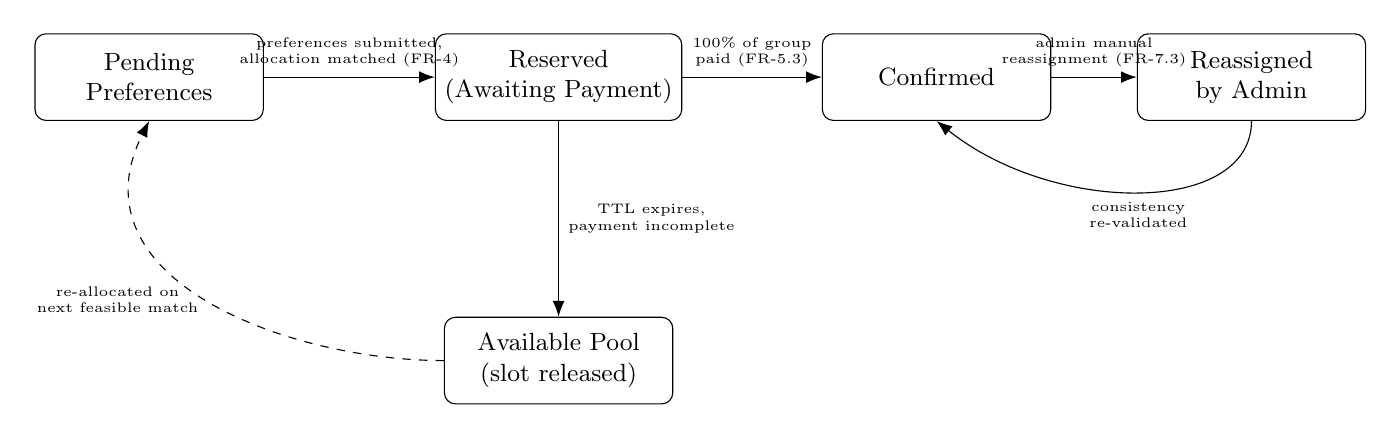
\begin{tikzpicture}[
    box/.style={rectangle, rounded corners, draw=black, minimum width=2.9cm, minimum height=1.1cm, align=center, font=\small},
    arrow/.style={-{Latex[length=2mm]}}
]
\node[box] (pending) at (0,0) {Pending\\Preferences};
\node[box] (reserved) at (5.2,0) {Reserved\\(Awaiting Payment)};
\node[box] (confirmed) at (10,0) {Confirmed};
\node[box] (reassigned) at (14,0) {Reassigned\\by Admin};
\node[box] (pool) at (5.2,-3.6) {Available Pool\\(slot released)};

\draw[arrow] (pending) -- node[above, font=\tiny, align=center] {preferences submitted,\\allocation matched (FR-4)} (reserved);
\draw[arrow] (reserved) -- node[above, font=\tiny, align=center] {100\% of group\\paid (FR-5.3)} (confirmed);
\draw[arrow] (confirmed) -- node[above, font=\tiny, align=center] {admin manual\\reassignment (FR-7.3)} (reassigned);
\draw[arrow] (reassigned.south) .. controls +(0,-1.2) and +(1.5,-1.2) .. node[below, font=\tiny, align=center] {consistency\\re-validated} (confirmed.south);
\draw[arrow] (reserved) -- node[right, font=\tiny, align=center] {TTL expires,\\payment incomplete} (pool);
\draw[arrow, dashed] (pool.west) .. controls +(-2,0) and +(-1,-2) .. node[left, font=\tiny, align=center] {re-allocated on\\next feasible match} (pending.south);
\end{tikzpicture}
\caption{Booking status state diagram, including TTL-driven release back to the available pool.}
\end{figure}

\subsection*{FR-7: Admin Module}
\begin{itemize}[leftmargin=1.2cm]
    \item \textbf{FR-7.1}: Admin can edit hostel, floor, cluster and room records and re-sync them from FretBox.
    \item \textbf{FR-7.2}: Admin can view all allocations, filtered by hostel, floor, cluster or payment status, and run payment reconciliation reports.
    \item \textbf{FR-7.3}: Admin can manually reassign or vacate a student or group, triggering allocation consistency checks.
\end{itemize}

% ============================================================
\chapter{External Interface Requirements}

\section{User Interfaces}
\begin{itemize}[leftmargin=1.2cm]
    \item \textbf{Landing / Auth}: login and signup with an imagery-led hero section.
    \item \textbf{Dashboard and Cluster Browser}: group status and profile summary, plus a card-based floor map with live occupancy badges.
    \item \textbf{Preference Ranking and Payment}: drag-to-rank cluster selection, followed by a Razorpay checkout with a per-member status checklist.
    \item \textbf{Admin Dashboard}: tabular management views with inline edit and override actions.
\end{itemize}

\section{Hardware Interfaces}
None --- any network-connected device with a browser.

\section{Software Interfaces}
\begin{longtable}{p{3.2cm}p{10.5cm}}
\toprule
\textbf{Interface} & \textbf{Purpose} \\
\midrule
FretBox & Source of student and hostel master data; imported, never hand-entered \\
PostgreSQL & Primary data store --- users, groups, hostel hierarchy, bookings, payments \\
Redis & Distributed locking for the allocation critical section; occupancy caching \\
Razorpay API & Payment order creation, checkout, and webhook-based verification \\
\bottomrule
\end{longtable}

\section{Communications Interfaces}
\begin{itemize}[leftmargin=1.2cm]
    \item REST over HTTPS (JSON) between the Next.js frontend and the FastAPI backend, plus a signature-verified Razorpay webhook for asynchronous payment confirmation and a scheduled FretBox data sync.
\end{itemize}

% ============================================================
\chapter{Non-Functional Requirements}

\section{Performance}
An allocation decision must resolve in under 500 ms under normal load, with at least 200 concurrent
booking attempts handled without double-allocation.

\section{Security}
\begin{itemize}[leftmargin=1.2cm]
    \item Passwords hashed with bcrypt; JWT tokens with expiry and a refresh flow; role-based access control on all admin endpoints.
    \item Razorpay payment signatures verified server-side before a payment is marked complete.
\end{itemize}

\section{Reliability \& Availability}
Reservation locks auto-expire (TTL, configurable, default 15 minutes) if payment is not completed,
releasing the slot back to the pool and preventing deadlock or starvation.

\section{Maintainability}
A layered backend (routers $\rightarrow$ services $\rightarrow$ repositories) isolates the allocation
algorithm as an independently testable module; hostel data is refreshed from FretBox by
configuration, not code change.

\section{Portability}
Fully containerized; runs identically on any Docker-enabled host via \texttt{docker compose up}.

\section{Usability}
Responsive design for mobile and desktop, following familiar booking-platform conventions to
minimise onboarding friction.

\section{Business Rules}
\begin{itemize}[leftmargin=1.2cm]
    \item A booking is Confirmed only when every group member's payment status is paid, and no group may exceed 4 members.
    \item Only an Admin or Warden may reassign a confirmed booking or edit master hostel data.
\end{itemize}

% ============================================================
\chapter{System Architecture (High-Level)}

The Next.js frontend communicates over REST/JSON (HTTPS) with the FastAPI backend, which contains
the routers, services and allocation engine. The backend persists to PostgreSQL, uses Redis for locks
and caching, imports master data from FretBox, and calls Razorpay for payments. All services are
orchestrated by Docker Compose.

\begin{figure}[h]
\centering
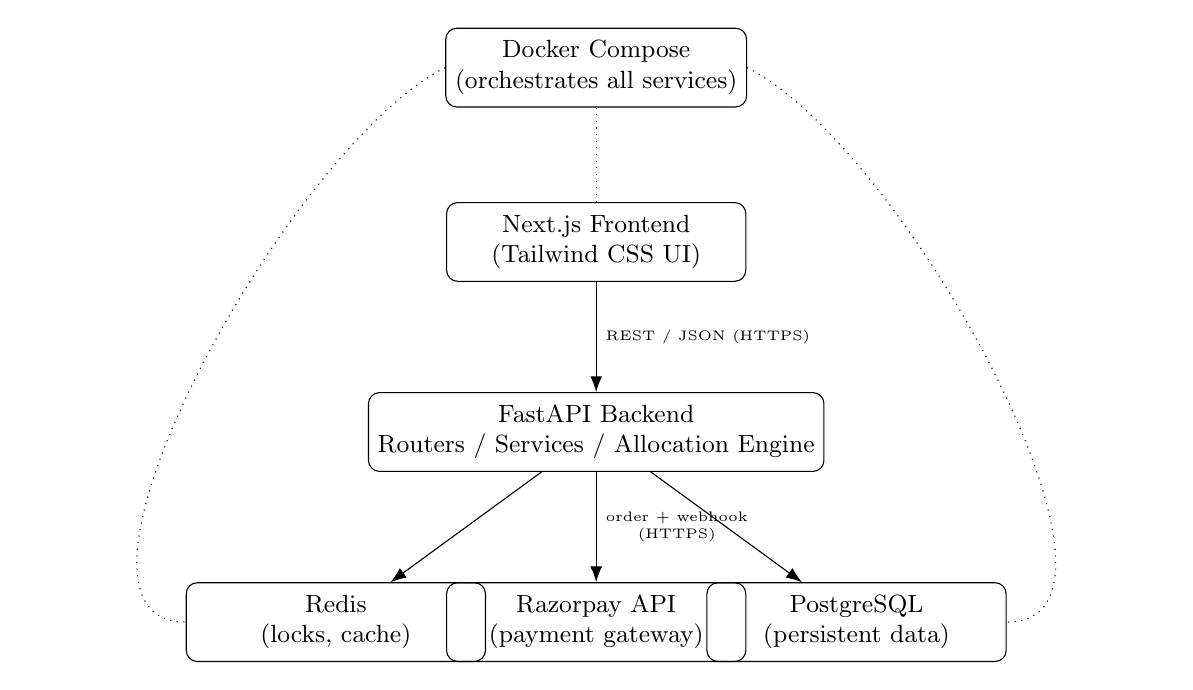
\begin{tikzpicture}[
    node distance=1.2cm and 1.2cm,
    box/.style={rectangle, rounded corners, draw=black, minimum width=3.8cm, minimum height=1cm, align=center, font=\small},
    arrow/.style={-{Latex[length=2mm]}}
]
\node[box] (compose) {Docker Compose\\(orchestrates all services)};
\node[box, below=of compose] (frontend) {Next.js Frontend\\(Tailwind CSS UI)};
\node[box, below=1.4cm of frontend] (backend) {FastAPI Backend\\Routers / Services / Allocation Engine};
\node[box, below left=1.4cm and -1.5cm of backend] (redis) {Redis\\(locks, cache)};
\node[box, below=1.4cm of backend] (razorpay) {Razorpay API\\(payment gateway)};
\node[box, below right=1.4cm and -1.5cm of backend] (postgres) {PostgreSQL\\(persistent data)};

\draw[arrow] (frontend) -- node[right, font=\tiny] {REST / JSON (HTTPS)} (backend);
\draw[arrow] (backend) -- node[right, font=\tiny, align=center] {order + webhook\\(HTTPS)} (razorpay);
\draw[arrow] (backend) -- (redis);
\draw[arrow] (backend) -- (postgres);
\draw[dotted] (compose) -- (frontend);
\draw[dotted] (compose.west) .. controls +(-2,-1) and +(-2,0) .. (redis.west);
\draw[dotted] (compose.east) .. controls +(2,-1) and +(2,0) .. (postgres.east);
\end{tikzpicture}
\caption{High-level system architecture and service communication.}
\end{figure}

% ============================================================
\chapter{Data Model (Entity Overview)}

\begin{longtable}{p{3.6cm}p{10cm}}
\toprule
\textbf{Entity} & \textbf{Key Attributes} \\
\midrule
User & id, name, roll\_no, email, password\_hash, role, gender, year, branch (synced from FretBox) \\
Group / GroupMember & group: id, code, leader\_id, size, status \textbar\ member: group\_id, user\_id, payment\_status \\
Hostel / Floor / Cluster / Room & hostel: id, name, gender, year \textbar\ floor: hostel\_id, floor\_number \textbar\ cluster: floor\_id, cluster\_number \textbar\ room: cluster\_id, room\_number, capacity=2, occupied\_count \\
Preference & id, group\_id, cluster\_id, rank \\
Booking / Payment & booking: id, group\_id, cluster\_id, room\_ids[], status, created\_at (FCFS) \textbar\ payment: id, user\_id, razorpay\_order\_id, amount, status \\
\bottomrule
\end{longtable}

% ============================================================
\chapter{Allocation Algorithm --- Detailed Logic}

Inputs: a group (size and ranked cluster preferences) and the current occupancy snapshot. For each
preferred cluster, in rank order:

\begin{enumerate}[leftmargin=1.2cm]
    \item Lock the cluster ID to prevent concurrent changes.
    \item Check occupancy against group size per FR-4.1 to FR-4.3: 4-member groups need both rooms empty; 3-member groups need the leader's room empty and the other empty or holding one occupant; 2-member groups need only the leader's room empty; singles need exactly one free seat.
    \item If it fits, create a Reserved (Awaiting Payment) booking, timestamp it for FCFS, and release the lock; if not, release the lock and try the next preference.
    \item If no preference fits, search all clusters for a free slot, or flag the group for Admin allocation.
    \item Once every member pays within the TTL the booking is Confirmed; otherwise it is released back to the pool.
\end{enumerate}

\begin{figure}[h]
\centering
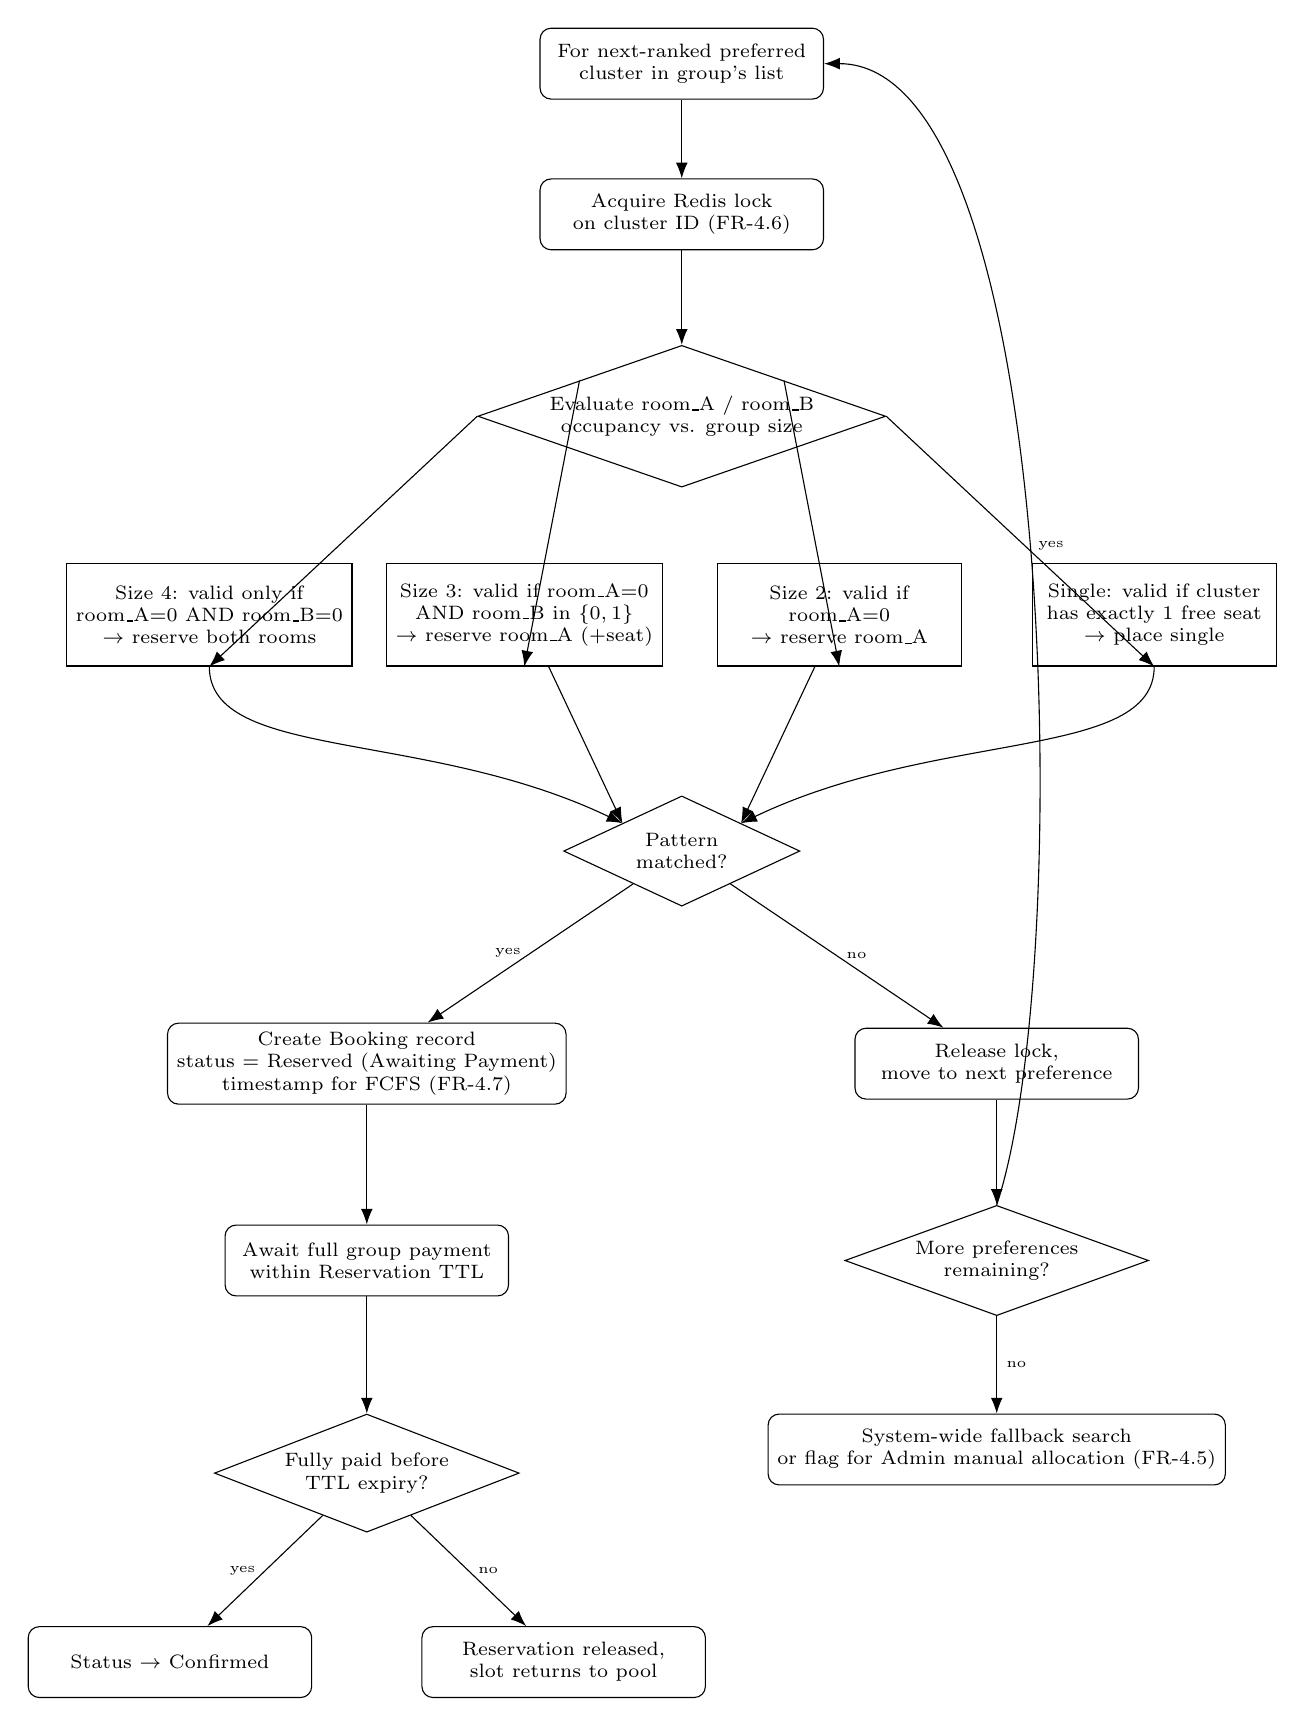
\begin{tikzpicture}[
    box/.style={rectangle, rounded corners, draw=black, minimum width=3.6cm, minimum height=0.9cm, align=center, font=\scriptsize},
    smallbox/.style={rectangle, draw=black, minimum width=3.1cm, minimum height=1.3cm, align=center, font=\scriptsize},
    decisionbox/.style={diamond, draw=black, aspect=3, align=center, font=\scriptsize, inner sep=1pt},
    arrow/.style={-{Latex[length=2mm]}}
]
\node[box] (start) at (0,17) {For next-ranked preferred\\cluster in group's list};
\node[box, below=1cm of start] (lock) {Acquire Redis lock\\on cluster ID (FR-4.6)};
\node[decisionbox, below=1.2cm of lock, minimum width=4.5cm, minimum height=1.8cm] (eval) {Evaluate room\_A / room\_B\\occupancy vs. group size};

\node[smallbox] (size4) at (-6,10) {Size 4: valid only if\\room\_A=0 AND room\_B=0\\$\rightarrow$ reserve both rooms};
\node[smallbox] (size3) at (-2,10) {Size 3: valid if room\_A=0\\AND room\_B in $\{0,1\}$\\$\rightarrow$ reserve room\_A (+seat)};
\node[smallbox] (size2) at (2,10) {Size 2: valid if\\room\_A=0\\$\rightarrow$ reserve room\_A};
\node[smallbox] (single) at (6,10) {Single: valid if cluster\\has exactly 1 free seat\\$\rightarrow$ place single};

\node[decisionbox, minimum width=3cm, minimum height=1.4cm] (matched) at (0,7) {Pattern\\matched?};
\node[box] (create) at (-4,4.3) {Create Booking record\\status = Reserved (Awaiting Payment)\\timestamp for FCFS (FR-4.7)};
\node[box] (release) at (4,4.3) {Release lock,\\move to next preference};
\node[decisionbox, minimum width=3.2cm, minimum height=1.4cm] (more) at (4,1.8) {More preferences\\remaining?};
\node[box] (fallback) at (4,-0.6) {System-wide fallback search\\or flag for Admin manual allocation (FR-4.5)};
\node[box] (await) at (-4,1.8) {Await full group payment\\within Reservation TTL};
\node[decisionbox, minimum width=3.4cm, minimum height=1.5cm] (paid) at (-4,-0.9) {Fully paid before\\TTL expiry?};
\node[box] (conf) at (-6.5,-3.3) {Status $\rightarrow$ Confirmed};
\node[box] (rel) at (-1.5,-3.3) {Reservation released,\\slot returns to pool};

\draw[arrow] (start) -- (lock);
\draw[arrow] (lock) -- (eval);
\draw[arrow] (eval.west) -- (size4.south);
\draw[arrow] (eval.north west) -- (size3.south);
\draw[arrow] (eval.north east) -- (size2.south);
\draw[arrow] (eval.east) -- (single.south);
\draw[arrow] (size4.south) .. controls +(0,-1.2) and +(-2.5,1.2) .. (matched.north west);
\draw[arrow] (size3) -- (matched.north west);
\draw[arrow] (size2) -- (matched.north east);
\draw[arrow] (single.south) .. controls +(0,-1.2) and +(2.5,1.2) .. (matched.north east);
\draw[arrow] (matched) -- node[left, font=\tiny] {yes} (create);
\draw[arrow] (matched) -- node[right, font=\tiny] {no} (release);
\draw[arrow] (release) -- (more);
\draw[arrow] (more) -- node[right, font=\tiny] {no} (fallback);
\draw[arrow] (more.north) .. controls +(1,3) and +(3,0) .. node[right, font=\tiny] {yes} (start.east);
\draw[arrow] (create) -- (await);
\draw[arrow] (await) -- (paid);
\draw[arrow] (paid) -- node[left, font=\tiny] {yes} (conf);
\draw[arrow] (paid) -- node[right, font=\tiny] {no} (rel);
\end{tikzpicture}
\caption{Allocation algorithm decision flow, evaluated per ranked cluster preference.}
\end{figure}

\textbf{Edge cases:} competing 3-member groups are resolved by FCFS booking-ready timestamp; a
single applicant with no matching seat in any preferred cluster falls back to a system-wide search
(FR-4.4).

% ============================================================
\chapter{Appendix}

\section{Tech Stack Summary}
\begin{longtable}{p{3.2cm}p{10.5cm}}
\toprule
\textbf{Layer} & \textbf{Technology} \\
\midrule
Frontend & Next.js (App Router), Tailwind CSS \\
Backend & FastAPI (Python), Pydantic, JWT (OAuth2 password flow) \\
Data & PostgreSQL (persistence), Redis (locking and cache), FretBox (master data source) \\
Integration / Deployment & Razorpay payments; Docker and Docker Compose \\
\bottomrule
\end{longtable}

\end{document}
